\chapter{State Space Analysis and Verification}
\label{chapter:analysis}

Consider the sample deployment shown in Figure \ref{fig:CT}. This is a 3-satellite cluster with each satellite consisting of an instance of a DREMS application. All satellites are deployed with the same component assembly and Satellite 1 is chosen as the cluster leader using a leader-election algorithm. 

\begin{figure}[htb]
	\centering
	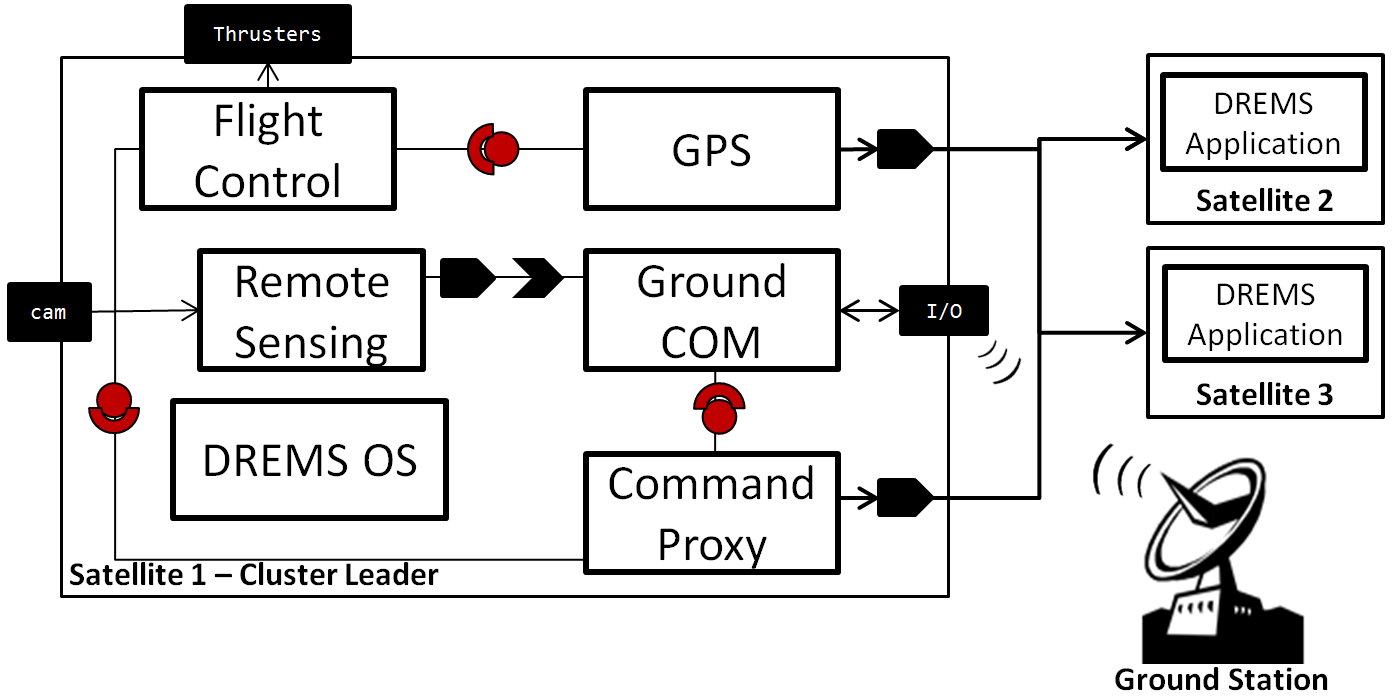
\includegraphics[width=\textwidth]{./img/Case_Study_Fixed.png}
	\caption{DREMS Application}
	\label{fig:CT}
\end{figure}

Each satellite consists of a set of sensor-dependent critical components required for both safe flight and remote sensing tasks. These components interact with physical sensor devices such as cameras, radar altimeters etc. to receive and process data periodically and transmit to a ground receiving station. The component \emph{Ground COM} behaves as the communication link between internal satellite components and the ground station. Periodically processed and encoded image data from the \emph{Remote Sensing} device is received by the Ground COM using a DDS-based \emph{publish-subscribe} scheme upon which the data is transmitted to the ground receiver. 

A more critical task in this deployment is maintaining the cluster attitude. This includes the relative position and acceleration of the satellites from each other with the satellites using a distributed but synchronized database to keep track of \emph{state vectors} of each other. A \emph{GPS} component periodically publishes a state vector to all satellites in the cluster. The GPS component uses its subscriber port to receive the equivalent vectors from other satellites. A \emph{Flight Control} component responsible for the integrity of the cluster flight uses an RMI interface to access the most recent vector metrics from GPS including metrics received from other satellites to calculate and maintain the flight trajectory. The Flight Control component does not fetch GPS information until all the satellites have published on the updated sensor data. 

Lastly, there are scenarios where the ground station will command the satellites in the cluster to perform a coordinated \emph{scatter}. This is a time-triggered critical event that is transmitted to the cluster leader. On receiving such a command, the Ground COM of Satellite 1 uses an interface on the \emph{Command Proxy} to publish this command to all satellites in the cluster. The command proxy uses a high-priority synchronous method invocation to communicate with the Flight Control component to trigger the scatter. Since the component-level scheduler is non-preemptive, the Flight Control cannot trash any operation that it would be executing at time $t_S$ when a scatter request is received from the Command Proxy. This motivates the need for accurate modeling of component interaction semantics to obtain conservative response-time results. 

\begin{figure}[htb]
	\centering
	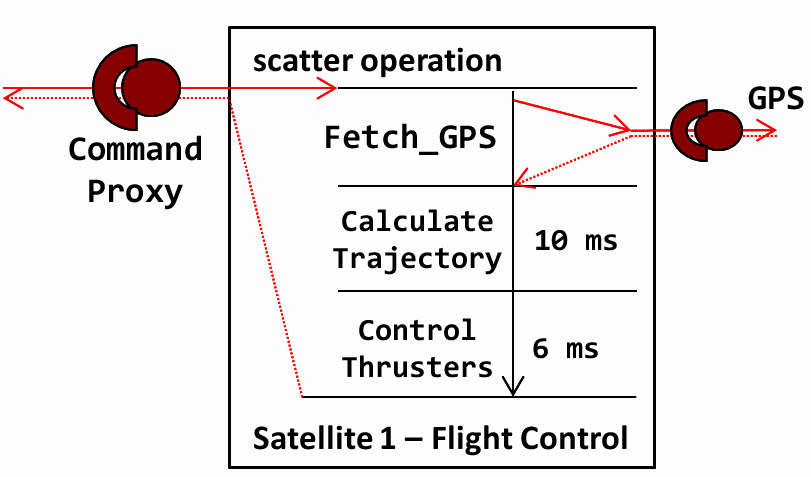
\includegraphics[width=0.7\textwidth]{./img/scatter.jpg}
	\caption{Scatter Operation}
	\label{fig:FLC}
\end{figure}

The abstract business logic \emph{steps} of the \emph{scatter} operation in the Flight Control is modeled as shown in Figure \ref{fig:FLC}. This operation is requested by the Command Proxy when a command is received from the ground station. For sake of simplicity, we have reduced this operation down to 3 distinct steps. The controller first obtains updated position vectors from the GPS component using the RMI interface. Notice the lack of a WCET for this interaction. This is because the GPS is scheduled on a separate temporal partition and the amount of time for which the Flight Control has to wait for the updated metrics is dependent on the time stamp at which the scatter command is received and also the state of the GPS component message queue. Once these metrics are received, the Flight Control calculates a new trajectory which is also the return arguments of this operation. This trajectory is passed down to the Command Proxy which publishes the leader's updated metrics to the rest of the satellites in the cluster. Once the trajectory is calculated, each Flight Control component interacts with the thrusters and maneuvers the satellites.  

The temporal partitioning schedule for this scenario consists of two broad minor frames each of length 100 msec. All satellite sensor components such as the camera and the GPS are grouped into sensor processes and assigned to the first temporal partition. This includes the image processing tasks undertaken by the Remote Sensing component, the vector publication and reception by the GPS component and the communication with the ground network. 

The Flight Control is assigned to partition 2 and is guaranteed to receive the newest vector data as it waits for the GPS component to update the database of state variables. The Ground COM and the Command Proxy component threads run at SYSTEM priority and are scheduled as and when required. In our case, we use a sporadic timer on the Ground COM component to trigger the sequence of interactions leading a scatter.

\section{State Space Analysis}

CPN Tools uses a built-in state space (SS) analysis tool to generate a bounded state space from an initialized CPN model. Exceptions caused by inconsistent token structures or incomplete arc bindings cause the tool to stop generation. However, it has been noted by the CPN Tools community that the built-in state space tool is inefficient with its search algorithm \cite{CPNTwoInterfaces} and therefore we also work with the ASAP tool \cite{ASAP} which is an extensible platform for advanced CPN state space analysis methods including optimized reduction techniques for large-scale applications. Thirdly, we also use the ASK-CTL \cite{ASK-CTL} model checking library, expressing state space properties using a CTL-style logic and exploiting strongly connected components for efficient state space searching. For smaller design models, we use observer places \cite{Alpern1989} in the CPN to \emph{collect} tokens that represent timing anomalies such as deadline violations. This makes the state space search easier as we simply look for nodes where the observer places are not empty. 

\subsection{Bounded State Space Generation}

Components in safety-critical DRE applications can be either sporadically or periodically triggered by an entity. A bounded state space generated in CPN Tools must be sufficiently large so that the lack of deadline violations or deadlocks or delayed response times \emph{during} this interval will guarantee safe operation throughout the lifetime of the components. This is important in order to gain confidence from the obtained results while not generating an infinite state space. 

\subsection{Deadline Violations and System-wide Deadlocks}

On a sufficiently large bounded state space, the analysis tool looks for specific behavioral patterns such as weakly-decreasing size of the component message queue. If requests from external components or timers pile up over time in the message queue, the responsible component is not scheduled for long enough time to be able to serve all the requests on time. This observation will also be supported by the detection of deadline violations or unusual blocking times. This is especially useful in identifying timing delays that propagate through successive hyperperiods in the temporal partition schedule. 

\begin{figure}[htb]
	\centering
	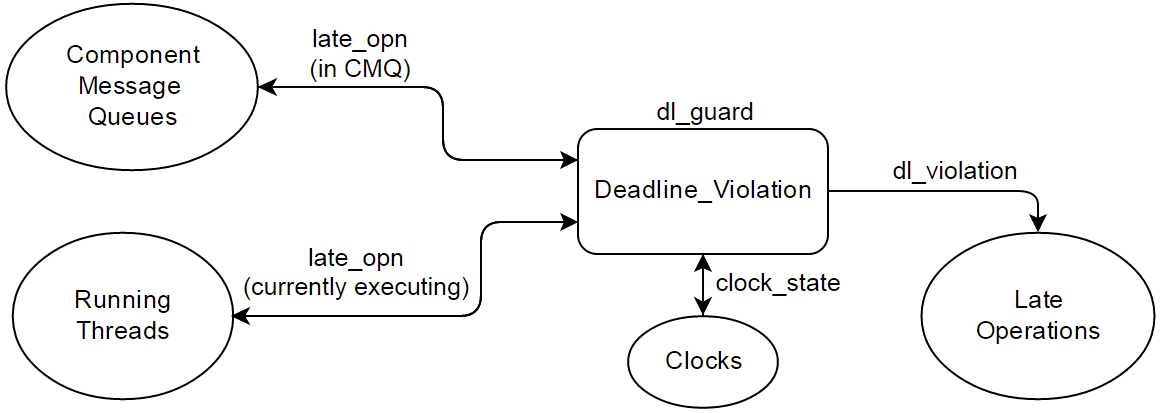
\includegraphics[width=\textwidth]{./img/Deadline_Violations.png}
	\caption{Deadline Violation Observer place}
	\label{fig:DL}
\end{figure}

As mentioned earlier, our model uses an observer place for deadline violation detection, especially in small/medium sized applications. A \emph{Deadline\_Violation} (Figure \ref{fig:DL}) transition fires at any point in time when the guard \emph{dl\_guard} is satisfied and arc bindings are realized with its input places. The transition observes the states of the currently running threads and the component message queues to identify deadline violations on operations that are either executing or waiting to execute. The \emph{dl\_violation} tokens in \emph{Late Operations} ($LO$) is of the form:

\begin{equation}
\label{eq:DLV}
LO = \ <Node_{name}, O_{name}, O_{ST}, \ O_{DLT}>
\end{equation}

where operation $O_{name}$ executing on computing node $Node_{name}$ started at time $O_{ST}$ and violated its deadline at time $O_{DLT}$. Since the component-level scheduler uses a non-preemptive scheme, this operation is still run to completion after the violated deadline. Delays like these propagate to the waiting operations in the message queue.

\begin{table}[h]
	\caption{Component Operations on Satellite 1}
	\label{table:AR}
	\begin{center}
		\begin{tabular}{ | c | p{1.0cm} | p{1.0cm} | p{1.0cm} | p{1.0cm} | p{1.0cm} | p{1.0cm} |}
			\hline
			Component & \multicolumn{1}{|c|}{Operation} & $Dl_{O}$ (ms) & $T_{NQ}$ (ms) & $T_{DQ}$ (ms) & $T_{FIN}$ (ms) & $T_{EXEC}$ (ms) \\ \hline
			GPS & \multicolumn{1}{|c|}{publish\_vector} & \multicolumn{1}{|c|}{10} & \multicolumn{1}{|c|}{0} & \multicolumn{1}{|c|}{0} & \multicolumn{1}{|c|}{8} & \multicolumn{1}{|c|}{8} \\ \hline
			GPS & \multicolumn{1}{|c|}{update\_dbs} & \multicolumn{1}{|c|}{18} & \multicolumn{1}{|c|}{20 (n/w delay)} & \multicolumn{1}{|c|}{20} & \multicolumn{1}{|c|}{36} & \multicolumn{1}{|c|}{16} \\ \hline
			Remote Sensing & \multicolumn{1}{|c|}{img\_process} & \multicolumn{1}{|c|}{90} & \multicolumn{1}{|c|}{0} & \multicolumn{1}{|c|}{12} & \multicolumn{1}{|c|}{80} & \multicolumn{1}{|c|}{80} \\ \hline
			Ground COM & \multicolumn{1}{|c|}{transmit\_imgs} & \multicolumn{1}{|c|}{20} & \multicolumn{1}{|c|}{80} & \multicolumn{1}{|c|}{80} & \multicolumn{1}{|c|}{95} & \multicolumn{1}{|c|}{15} \\ \hline
			Ground COM & \multicolumn{1}{|c|}{scatter\_cmd} & \multicolumn{1}{|c|}{200} & \multicolumn{1}{|c|}{120} & \multicolumn{1}{|c|}{120} & \multicolumn{1}{|c|}{315} & \multicolumn{1}{|c|}{195} \\ \hline
			Command Proxy & \multicolumn{1}{|c|}{notify\_cmd} & \multicolumn{1}{|c|}{200} & \multicolumn{1}{|c|}{132} & \multicolumn{1}{|c|}{132} & \multicolumn{1}{|c|}{142} & \multicolumn{1}{|c|}{10} \\ \hline
			Flight Control & \multicolumn{1}{|c|}{calc\_trj} & \multicolumn{1}{|c|}{45} & \multicolumn{1}{|c|}{100} & \multicolumn{1}{|c|}{100} & \multicolumn{1}{|c|}{150} & \multicolumn{1}{|c|}{50} \\ \hline
			Flight Control & \multicolumn{1}{|c|}{scatter} & \multicolumn{1}{|c|}{200} & \multicolumn{1}{|c|}{142} & \multicolumn{1}{|c|}{150} & \multicolumn{1}{|c|}{305} & \multicolumn{1}{|c|}{163} \\ \hline
			
			
		\end{tabular}
	\end{center}
\end{table}

For a large state space, using observer places is not the most efficient approach as the accumulated violation tokens themselves contribute to the state space. An easy fix to this challenge is to stop generating state space nodes after the detection of the first violation. However, if all system violations need to be recorded, then instead of using observer places, we query the state space of transition firings to find \emph{binding elements} that indirectly suggest a violation.

System-wide deadlocks are caused by the inability of the OS schedulers (on all nodes) to schedule any component thread. This can be caused by situations where a set of executing threads are indefinitely blocked on each other because of cyclic dependencies in the interactions. Deadlocks can identified by checking the leaf nodes of the bounded state space for \emph{dead transitions} that are unable to fire. Alternatively, the tokens in \emph{Component Interactions} are analyzed to identify cyclic dependencies and provide warnings to possible deadlocks. Such queries are useful in large component assemblies where mutually blocking dependencies are not immediately perceivable. 

\begin{figure}[htb]
	\centering
	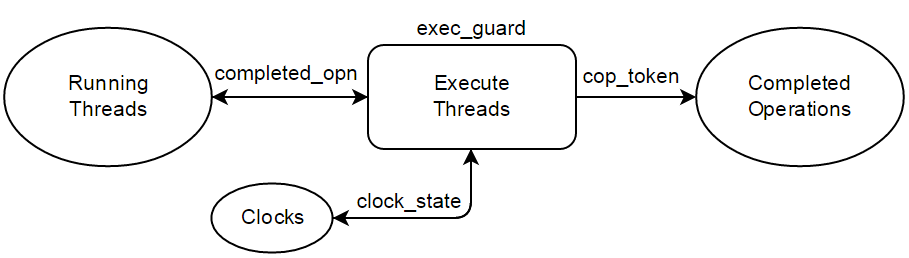
\includegraphics[width=\textwidth]{./img/Response_Times.png}
	\caption{Response-time Analysis}
	\label{fig:COP}
\end{figure}

\subsection{Response-time Analysis}

Response-times are measured by observing completed operations. Similar to deadline violations, an observer place \emph{Completed Operations} (Figure \ref{fig:COP}) accumulates all operation requests completed by component threads on all nodes. The structure of this data is similar to equation \ref{eq:DLV} except we replace $O_{DLT}$ with the end-time of the operation $O_{ET}$.

For a known trigger operation and an expected response/actuation, we used state space queries to identify the (1) earliest completion of the trigger operation and the (2) latest completion of a response operation. These operations are possibly running on different components, temporal partitions or nodes. To keep a check on the state space for large models, we simply observe the bindings of the transition \emph{Execute Thread} to gather a list of completed operations, ordered by $O_{ET}$.

\subsection{Search Results}

Table \ref{table:AR} shows some worst-case execution time results from state space analysis on each component thread on Satellite 1. Each operation request is enqueued into the component message queue at $T_{NQ}$. A dispatcher thread dequeues this request at $T_{DQ}$ and schedules an operation for execution. Delays in the dequeue can be caused due to the non-preemptive nature of the component-level scheduling. Once scheduled, the component executor thread sequentially executes the steps in each operation to completion at time stamp $T_{FIN}$ leading to an overall execution time of $T_{EXEC}$ measured starting from $T_{NQ}$. 

Significant worst-case network delays are assumed between interacting components that are distributed. For instance, the GPS component on each node finishes publishing sensor data at time stamp 8 ms but the GPS components on other nodes do not notice the subscription token in the message queues till $T_{NQ} = 20 ms$. Also, the synchronous dependency of the Flight Control component with the GPS component is a sign of poor design as a scatter command received in partition 2 of one hyperperiod will most likely finish only a hyperperiod later as the updated GPS coordinates are queried. 

\subsection{Incomplete Designs}

In order to integrate this analysis approach into early stages of component-based design, we have looked into scenarios where this work is appropriate. As mentioned in Section \ref{subsec:Operation_Deadlines}, a component thread derives its deadlines from the operations it executes. These operations are triggered by requests from external entities with varying priorities. Identifying the optimal priority-assignment scheme for a set of component threads is non-trivial due to these variations. However, initial designs are often specified by timing requirements between system entities. Therefore, for scenarios where the developers are aware of minimum timing requirements but not thread execution orders or OS-level priorities, we have applied this approach to identify partial thread execution orders to refine incomplete designs. 

Consider a sample application that consists of 6 components servicing operation requests. Components threads 1, 2, and 3 are assigned to Partition 1 and threads 4, 5, and 6 are assigned to Partition 2. The thread priorities and execution orders are unknown. Each component is triggered by a timer once every major frame, taking up to 8 ms to complete the callback operation. Assuming a designer requires that operation 3 (handled by thread 3) must complete before 20 ms and operation 5 (handled by thread 5) must complete before 60 ms from the start of the schedule, the analysis will provide a partial thread execution order that satisfies these requirements. To facilitate this, we assign all the relevant threads equal priorities. If all the triggering timers expire at the beginning of the partition schedule, then all component threads become eligible for execution and the OS scheduler uses a non-deterministic round-robin scheduling scheme. By querying the bounded state space that encapsulates this behavior, we arrive at a partial thread scheduling order that satisfies our requirements e.g. thread 3 is scheduled first in partition 1 and thread 5 is scheduled first in partition 2.

\subsection{Discussion}

\subsubsection{Conservative Results}

Using estimates of worst-case execution time for component operations is motivated by the need to make exaggerated assumptions about the system behavior. Pessimistic estimates are a necessary requirement when verifying safety-critical DRE systems. Schedulability analysis with such assumptions should strictly provide conservative results. This means that:

\begin{itemize}
	\item If the analysis results show the possibility of a deadline violation but the deployed system does not, the obtained result is a conservative one as it assumes worst-case behavior. 
	
	\item If the analysis results do not show any timing violations but the deployed system violates response time requirements, deadlines etc., then the analysis does not provide a conservative result and has failed to verify system behavior.
\end{itemize}

In order to guarantee conservative results, the analysis must include worst-case behaviors of all system-level threads that run at higher priority than component threads and are not necessarily modeled by the design-time tools. These threads can be grouped into a set of critical processes with approximations made to simulate the behavior of system-level threads such as (1) globally periodic CPU utilization, (2) CPU utilization for some WCET per partition etc. The best approximation is chosen based on the expected behavior of such critical processes. Best-effort processes are ignored as they always run at a priority lower than the lowest-priority component thread.

\subsubsection{Scalability}
One of the main concerns in comprehensive design-time analysis of this kind is scalability. As the determinism in the initial design increases, the number of possible behaviors and therefore the size of the state space decreases. In essence, the effort required for the analysis to be useful to the designer is dependent heavily on the initial design itself. Increasing the number of equally prioritized components will exponentially increase the number of state space nodes required to accumulate the set of behaviors that are exhibited by the components. In \cite{MoDeVVa}, we presented results showing our analysis model scaling well for medium-sized applications tested up to a 100 mixed-criticality components distributed on up to 5 computing nodes. Although these results were based on design models that made some unrealistic assumptions e.g. 100 timers expiring at the same time and triggering interactions, we have used some heuristics to reduce the generated state space and improve the performance of the search methods. 
\paragraph{Symmetry}
One of the main advantages of using component-based design for complex systems is reusability. It is not unusual to deploy instances of the same application with the same component assembly on multiple computing nodes. If these applications are deployed on symmetrical nodes, the observed state space of behaviors are also symmetrical. To enable efficient search through symmetrical state spaces, we use symmetry-based state space reduction techniques \cite{Kristensen2000} to improve the performance. In Figure \ref{fig:hlcpn}, to model 100 timers, we moved from using 100 colored tokens in the \emph{Timers} place to using a single token which is a list consisting of a 100 elements. This way, when multiple timers expire, a single transition firing handles all the expiries across all nodes (a single state change) instead of multiple transition firings leading to multiple new states. This works well when a single instance of an application is deployed on several computing nodes with little non-determinism. The non-determinism caused by the OS-level scheduling of components and component-level operation request collisions still cause the state space to grow across symmetric nodes. 
\paragraph{ASAP Tool}
The CPN Tools GUI contributes to inefficient performance of state space generation for large CPN models. This is significantly improved by using the ASAP \cite{ASAP} analysis tool. The tool provides for several search algorithms and state space reduction techniques such as the \emph{sweep-line method} \cite{Christensen2001} which deletes already visited state space nodes from memory, forcing on-the-fly verification of temporal properties. One of the disadvantages of using such heuristics is the run-time cost incurred by backward-generation of states when a backtrace for a violation is required. However, if a path from the initial state to an inconsistent state is not desired, a combination of this method and the symmetry method reduces the state space and improves verification performance. 

\section{Modeling and Analysis Improvements}
\label{sec:Improvements}

\subsection{Problem Statement}

The CPN analysis work presented in \cite{kumar2014colored} has some limitations. The clock values in the distributed set of computing nodes progress by a fixed amount of time regardless of the pace of execution. This is one of the primary causes of state space explosion since many of the intermediate states between \emph{interesting} events, though uneventful, are still recorded by the state space generation. For instance, in a temporal partition spanning 100 ms, even if a thread executes for 5 ms and the rest of the partition is empty, then if the clock progresses at a 1 ms rate, a 100 states are recorded in the state space when there are atmost 5-7 interesting events in this interval. For a larger set of distributed interacting components, this can become a problem. Also, for distributed scenarios where multiple instance of a set of applications are executed in parallel, in independent computers, our CPN modeling methodology isn't efficient, leading to a tree of parallel executions even when the distributed computers are independent i.e. the computers can be synchronously progressed. The goal of this work is to mitigate such analysis issues and arrive at a more efficient and scalable analysis model. 

\subsection{Outline of Solution}
Improving the performance of our CPN analysis method required the evaluation of our existing results to identify how the state space generation worked. The state space of CPN is a tree of CPN \emph{markings}, where each marking is a data structure representing the tokens in all it's places. So, our goal is to reduce the number of markings accumulated in the CPN i.e. the number of distinct states of interest. This required us to evaluate our representation of time. Using time as a fixed-step monotonically increasing entity means that the CPN place managing time would always contain a new \emph{clock token}, therefore forcing the CPN marking to become a part of the state space.

To alleviate this issue, we modeled time as a dynamically changing variable, where the changes are strategically forced \emph{time jumps} instead of a statically increasing clock value. Similarly, our data structure representation for distributed deployments i.e. using unordered token sets instead of ordered lists, enabled our earlier CPN models to nondeterministically choose one of the various distributed nodes to execute, generating a exponentially increasing tree of execution orders. Once we moved to representing our distributed hardware nodes as a list, the execution engine iteratively executing the analysis on each node in the list, leading to one execution order instead of a tree. 

Such issues are resolved with our analysis improvements, reported in \cite{SEUS}. We modified the timing analysis model to allow dynamic time progression i.e. the clocks (one for each computing node) in the CPN model do not progress at a constant rate but instead experience \emph{time jumps} to the next interesting time step e.g. next timer expiry, end of partition or next scheduling preempt point. This makes the system execution progress at a much higher rate and reduces the overall number of states being recorded in the state space. We also adjusted our modeling concepts when describing distributed deployments. We experienced needless state space explosions as a consequence of using CPN semantics when modeling distributed computers. If the computers are modeled as an aggregate of independent CPN tokens, then the CPN transition that progresses the execution in each computer is independent, leading to a potential $C!$ different orders for $C$ computers. For instance, 4 distributed computers leads to 24 possible execution orders displayed by the transition responsible for \emph{picking} the next computer to evaluate and progress. We alleviate this issue by assuming that all computers in a distributed scenarios have synchronized clocks and execute simultaneously leading to a synchronous progress. This is done by maintaining the state of each computer in a \emph{list} instead of an unordered aggregate. This approach is inspired by the symmetry method for state space reduction \cite{Kristensen2000}. These improvements are evaluated in \cite{SEUS}, where we detail our solutions with motivating examples. 

\subsection{Handling Time}
\label{handling_time}

The CPN-based analysis consists of executing a simulation of the model and constructing a state space data structure for the system (for a finite horizon), and then performing queries on this data structure. This is automated by CPN Tools. The first improvement over the basic CPN approach is in how we handle time. Although it is true that CPN and similar extensions to Petri Nets such as Timed Petri Nets inherently have modeling concepts for simulation time, we explicitly model time as an integer-valued \emph{clock} color token in CPN. There are several reasons for this choice. 

Firstly, this is an extension to our previous arguments about choosing Colored Petri Nets. Modeling the OS scheduler clock as a colored token allows for extensions to its data structure such as (1) intermediate time stamps and internal state variables, and (2) adding temporal partitioning schemes like the (time-partitioned) ARINC-653 \cite{ARINC-653} scheduling model (Figure \ref{fig:clock}). 

\begin{figure}[h]
	\centering
	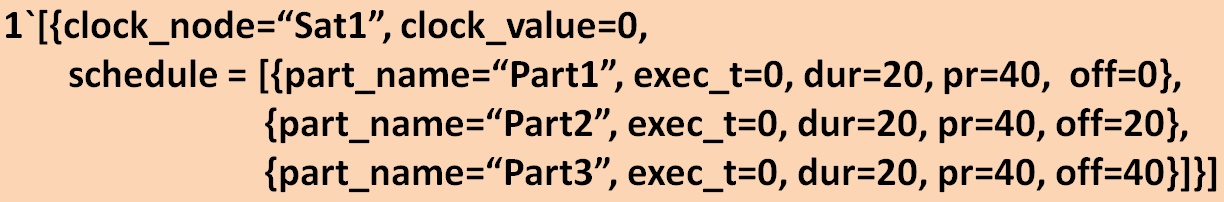
\includegraphics[width=0.7\textwidth]{./img/clock}
	\caption{A Clock Token with Temporal Partitioning}
	\label{fig:clock}
\end{figure}

These extended data structure fields can be more easily manipulated and used by the model transitions during state changes, allowing for richer modeling concepts that would not be easily attainable using token representations provided by Timed Petri Nets. The ability to pack colored tokens with rich data structures also reduces the total number of colors required by the complete model. This quantitative measure directly influences the reduced size of the resultant state space. The downside of this approach to modeling is that we have to choose a time quantum. But in practical systems this is usually not a problem, as the low-level scheduling decisions are taken by an OS scheduler based on a time scale with a finite resolution. We have chosen 1 msec as the quantum (corresponding to the typical 1KHz scheduler in Linux), but it can be easily changed. 

Secondly, modeling time as a token allows for smarter time progression schemes that can be applied to control the pace of simulation. If we did not have such control over time, the number of states recorded for this color token would eventually explode and itself contribute to a large state space. In order to manage this complexity, we have devised some appropriate \emph{time jumps} in specific simulation scenarios. 

If the rate at which time progresses does not change, then for a 1 msec time resolution, \emph{S} seconds of activity will generate a state space of size: $SS_{size} = \sum\limits_{i=1}^{S*1000} TF_{t_i}$ where $TF_{t_i}$ is the number of state-changing CPN transition firings between $t_i$ and $t_{i+1}$. This large state space includes intervals of time where there is no thread activity to analyze either due to lack of operation requests, lack of ready threads for scheduling, or due to temporal partitioning. During such idle periods, it is prudent to allow the analysis engine to \emph{fast-forward} time either to (1) the next node-specific clock tick, (2) the next global timer expiry event, or (3) the next activation of the node-specific temporal partition (whichever is earliest and most relevant). This ensures that the generated state space tree is devoid of nodes where there is no thread activity.

\begin{figure}[h]
	\centering
	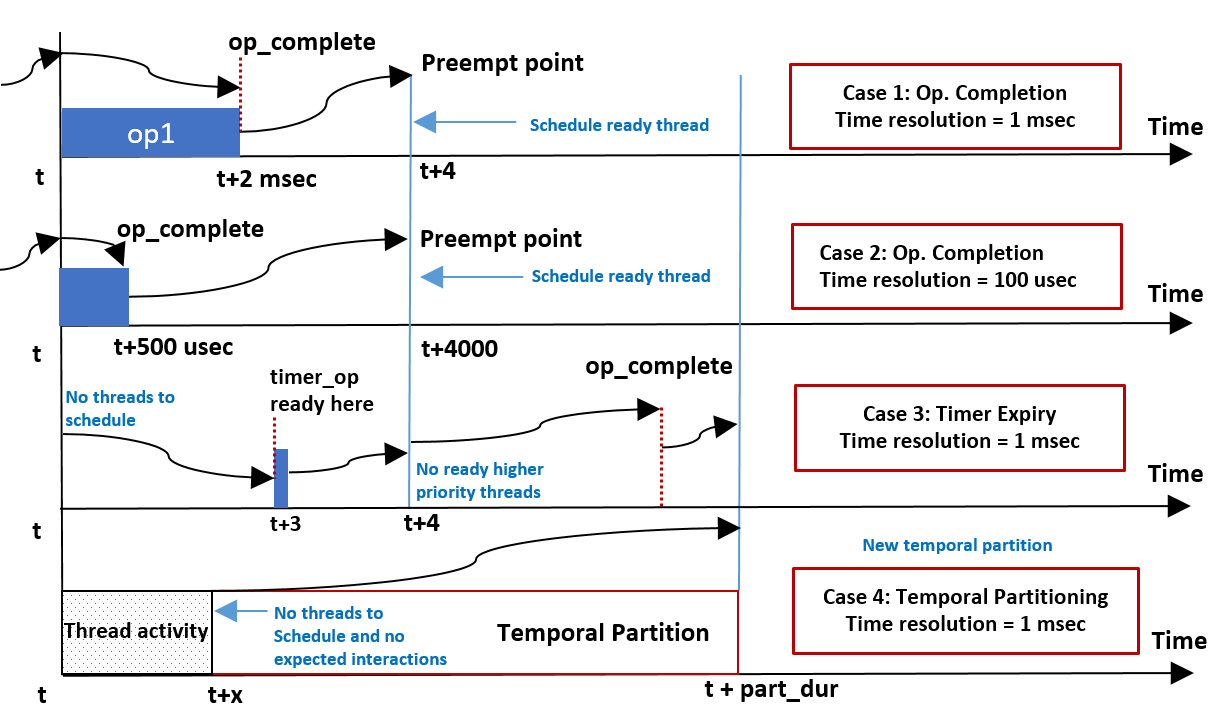
\includegraphics[width=\textwidth]{./img/time}
	\caption{Dynamic Time Progression}
	\label{fig:time}
\end{figure}

Figure \ref{fig:time} illustrates these time jumps using 4 scenarios. Assuming the scheduler clock ticks every 4 msec, Case 1 shows how time progression is handled when an operation completes 2 msec into its thread execution. At time t, the model identifies the duration of time left for an operation to complete. If this duration is earlier than the next preempt point, then there is no need to progress time in 1 msec increments as no thread can preempt this currently running thread till time t + 4 msec. Therefore, the \emph{clock\_value} in Figure \ref{fig:clock} progresses to time t + 2 msec, where the model handles the implications of the completed operation. This includes possibly new interactions and operation requests triggered in other components. Then, time is forced to progress to the next preempt point where a new candidate thread is scheduled. This same scenario is illustrated in Case 2 when the time resolution is increased to 100 usec instead of 1 msec. Notice that the number of steps taken to reach the preempt point are the same, showing how the state space doesn't have to explode simply because the time resolution is increased. Case 3 illustrates the scenario where at time t, the scheduler has no ready threads to schedule since there are no pending operation requests but at time t + 3 msec, a component timer expires, triggering an operation into execution. Since timers are maintained in a global list, each time the \emph{Progress\_Time} transition checks its firing conditions, it checks all possible timers that can expiry before the next preempt point. So, at time t when no threads are scheduled, the model immediately jumps to time t + 3. This scenario also shows that if the triggered operation does not complete before the preempt point \emph{and} there are no other ready threads or timer expiries that can be scheduled, the clock value jumps to the operation completion. It must be noted here that this case is valid only because the DREMS architecture we have considered uses a non-preemptive operation scheduling scheme. Lastly, Case 4 shows time jumps working with temporal partitioning. At some time t + x, the model realizes the absence of ready threads and does not foresee any interaction requests from other components, then it safely jumps to the end of the partition without stepping forward in 1 msec increments. This time progression directly shows how the state space of the system execution reduces while still preserving the expected execution order, justifying our choice of modeling time as a colored token using CPN. 

\subsection{Distributed Deployment} 
\label{distributed_deployment}

The second structural change to the analysis model is in how distributed deployments are modeled and simulated. Early designs on modeling and analysis of distributed application deployments \cite{kumar2014colored} included a unique token per CPN place for each hardware node in the scenario. Since the individual \emph{node} tokens are independent and unordered, there is nondeterminism in the transition bindings when choosing a hardware node to schedule threads in. For instance, if there are 2 hardware nodes in the deployment with ready threads on both nodes, then either node can be chosen first for scheduling threads leading to two possible variations of the model execution trace. Therefore the generated state space would exponentially grow for each new hardware node. In order to reduce this state space and improve the search efficiency, we have merged hardware node tokens into a single \emph{list} of tokens instead of a unassociated grouping of individual node tokens. This approach is inspired by the symmetry method for state space reduction \cite{Kristensen2000}.

\begin{figure}[h]
	\centering
	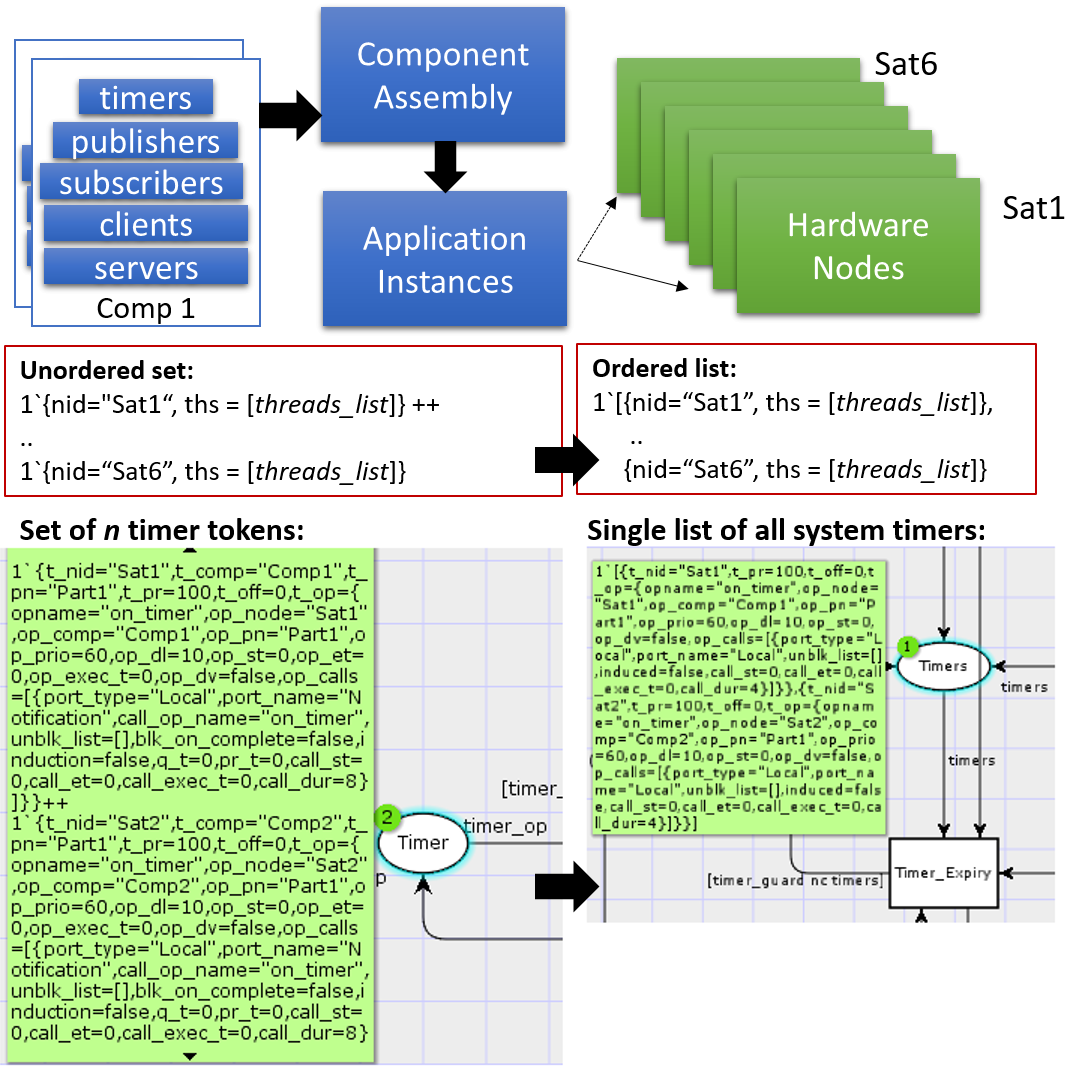
\includegraphics[width=0.8\textwidth]{./img/dd}
	\caption{Structural Reductions in CPN}
	\label{fig:dd}
\end{figure}

Figure \ref{fig:dd} illustrates this structural reduction. Consider a distributed deployment scenario with an instance of a DREMS application deployed on each hardware node, Sat1 through Sat6. Components \emph{Comp1} and \emph{Comp2} are triggered by timers, eventually leading to the execution of component operations (modeled as shown in Figure \ref{fig:ebnf}). If all the timer tokens in the system were modeled individually, the transition \emph{Timer\_Expiry} would non-deterministically choose one of the two timer tokens that are ready to expire at \emph{t=0}. However, if the timers are maintained as a single list, then this transition (1) consumes the entire list, (2) identifies all timers that are ready to expire, (3) evaluates the timer expiration function on all ready timers, (4) propagates the output \emph{operation} tokens to the relevant component message queues in a single firing. This greatly reduces the tree of possible transition firings and therefore the resultant state space. Also, if there is no non-determinism in the entire system, i.e., there is a distinct ordering of thread execution, then this model can be scaled up with instantiating the application on new hardware nodes with no increase in state space size. This is because all of the relevant tokens on all nodes are maintained as a single list that is completely handled by a single transition firing. 

An important implication of the above structural reduction is that the simulation of the entire system now progresses in synchronous steps. This means that at time 0, all the timers in all hardware nodes that are ready to expire will expire in a single step. Following this, all operations in all component message queues of all these nodes are evaluated together and appropriate component executor threads are scheduled together. When these threads execute, time progresses as described in Section \ref{handling_time}, moving forward by the minimum amount of time that can be fast-forwarded.

\newpage
\section{Investigating Advanced State Space Analysis Methods}

\subsection{Problem Statement}
State space analysis techniques have been successfully applied with Colored Petri Nets in a variety of practical scenarios and industrial use cases \cite{CPN_0}, \cite{CPN_1}. The basic idea here is to compute all reachable states of the modeled concurrent system and derive a directed graph called the state space. The graph represents the tree of possible executions that the system can take from an initial state. It is possible from this directed graph to verify behavioral properties such as queue overflows, deadline violations, system-wide deadlocks and even derive counterexamples when arriving at undesired states. 

Advanced state space analysis techniques arise from the need for efficient space space searching algorithms. State space analysis is challenged by time, memory, and computational power. Large state spaces require large CPU RAM and efficient search methodologies to quickly arrive at a useful result. With increasingly complexity in system designs, the number of state variables to store in memory also increases. Our problem here is to identify and apply advanced state space analysis techniques, applicable in the context of our CPN model and available as tested analysis tools that mitigate such complexities in state space analysis. This will help improve the scalability of our model and also reduce the memory footprint of the analysis. 

\subsection{Outline of Solution}

The variety of CPN-specific state space reduction techniques \cite{CPN_Sweepline}, \cite{CPN_Symmetry} developed in recent times has significantly broadened the class of systems that can be verified. In order to easily apply such techniques to our analysis model, we use the ASAP \cite{ASAP} analysis tool. The tool provides for several search algorithms and state space reduction techniques such as the \emph{sweep-line method} \cite{Christensen2001} which deletes already visited state space nodes from memory, forcing on-the-fly verification of temporal properties. The main advantage of such techniques is the amount of memory required by the analysis to verify useful properties for large models. 

The sweep line method for state space reduction is used to check for important safety properties such as lack of deadlocks, timing violations etc. using user-defined model-specific queries. Practical results enumerated in \cite{Christensen2001} show improvements in time and memory requirements for generating and verifying bounded state spaces. The method relies of discarding generated states on-the-fly by performing verification checks during state space generation time. Any state that does not violate system properties can be safely deleted. Another advantage of this method compared to similar reduction methods such as bit-state hashing \cite{CPN_Bitstate_Hashing} is that a complete state space search is guaranteed. 

\subsection{Evaluation of Solution}
We will evaluate these advanced state space analysis methods by comparing the obtained results with our basic state space analysis in CPN Tools. Using several criteria such as state space generation time, state space query generation, query processing time, memory usage etc., we can generate a comparison table to show the overall improvements in the analysis workflow. Advanced analysis techniques are usually accompanied by some expertise requirements that can be masked by nicely designed analysis tools. Our goal with ASAP is to use a model-driven approach to enable advanced analysis methods that does not require much expertise. With ASAP, we are able to generate verification project templates i.e. building blocks much like Simulink that are wired up together and provide an interface to the low-level analysis engine. Therefore, evaluation of this work requires both the evaluation of the advanced methods applied, and the tool used. As for the analysis methods applied, it is important to ensure that the state space tree, with all of the applied analysis heuristics, is still sufficiently probed when searching for system properties. Heuristics that enable state space analysis but only by partially checking the tree can lead the case where the state space analysis does not identify timing errors because of the incomplete search. This will be checked with negative test cases where the design model is known to be flawed; if the results from ASAP identify injected timing errors for all test cases, then the analysis is sound. 

\subsection{Contributions}
These methods were evaluated on our CPN analysis method and the results were presented in \cite{SEUS}. We used a large and diverse 100 component-based application for our testing. Using the CPN Tools' built-in state space analysis tool, a bounded state space of thread activity was generated. The state space generation took 36 minutes on a typical x86 laptop. We imported the same CPN analysis model onto ASAP and performed on-the-fly verification checks for lack of dead states in the analysis model for the same bounded state space. The on-the-fly verification, without any graphical interface overheads, took less than 10 minutes to compute a lack of system-wide deadlocks. It must be noted here that this improved result is due to not only because of the efficient state space search but also because of symmetry-based structural reduction discussed in the previous section.

In order to illustrate the utility of such state space reduction techniques, we consider a large-scale deployment. Figure \ref{fig:gm} shows the generated CPN model for a domain-specific DREMS application. This is a scaled-up variant of several satellite cluster examples we have used in previous publications \cite{DREMS13Software, kumar2014colored}. The example consists of a group of communicating satellites hosting DREMS applications. The component assembly for this application consists of 100 interacting components distributed across 10 computing nodes, many of which are triggered by infrastructural timers. Notice in Figure \ref{fig:gm} how there is only one token in each of the main CPN places, as described in Section \ref{distributed_deployment}. All of the component timers are appended to the list maintained in \emph{Timers} place. Similarly, all node-specific clock tokens are maintained in place \emph{Clocks}.  

\begin{figure}[h]
	\centering
	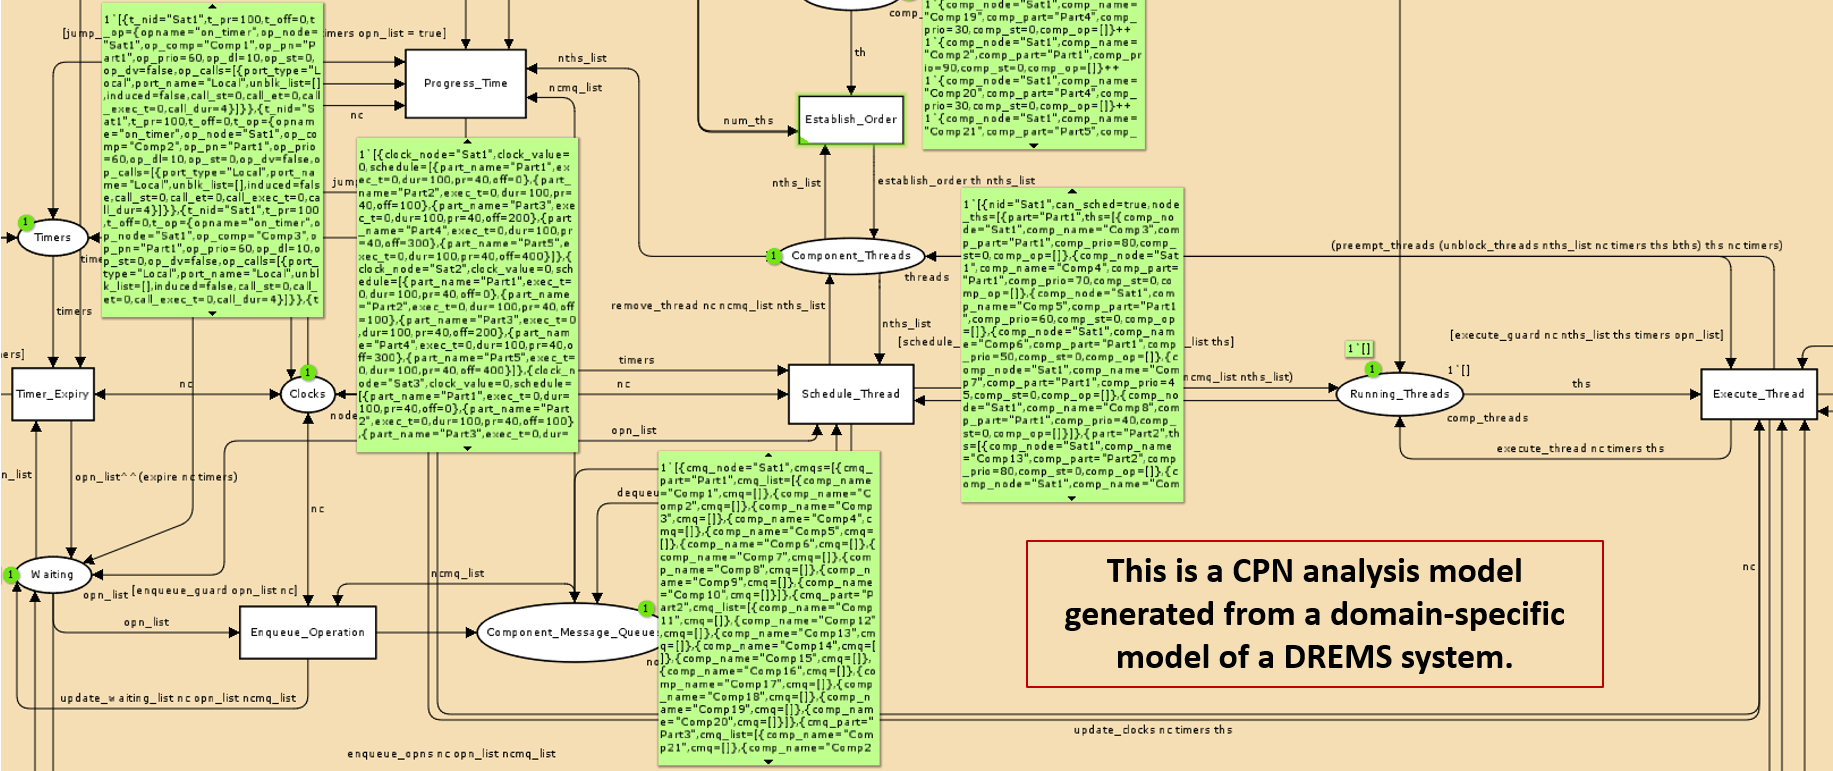
\includegraphics[width=\textwidth]{./img/Generated_Model}
	\caption{Generated CPN model for a Distributed Application Deployment}
	\label{fig:gm}
\end{figure}

At time \emph{t=0}, before the simulation is kicked off, the transition \emph{Establish\_Order} generates the powerset of thread execution orders that are possible given the configuration of the clock token. This may be a potentially large set depending on the number of threads of equal priority in each partition. Once this tree of possible orders is established, the complete set of timers that are ready to expire are evaluated. Each timer expiry manifests as an operation request and each callback operation modeled using the grammar shown in Figure \ref{fig:BL_Model}. Once the operations are ready to execute, the highest priority component thread with a pending operation request is chosen for execution. This thread scheduling happens on all hardware nodes. When each thread executes, new interactions may occur as a consequence of the execution. For instance, if a component thread executes a timer operation in which the component publishes on a global topic, the consequence of this action would include a set of callback operation requests on all components that contain subscribers to that global topic. Lastly, all running threads are evaluated to identify the minimum amount of time that can be safely fast-forwarded in each node. If the running component threads are independent or symmetrical, then the maximum possible time progression is up to the end of the temporal partition. Note here that temporal partition in the deployment can be set to an empty list which simply removes the  partitioning constraint and treats all component threads on a node as candidate threads for execution. The above sequence of transitions repeat for as long as there is a timer expiry, a pending operation request or an unfinished component interaction. 

\begin{figure}[h]
	\centering
	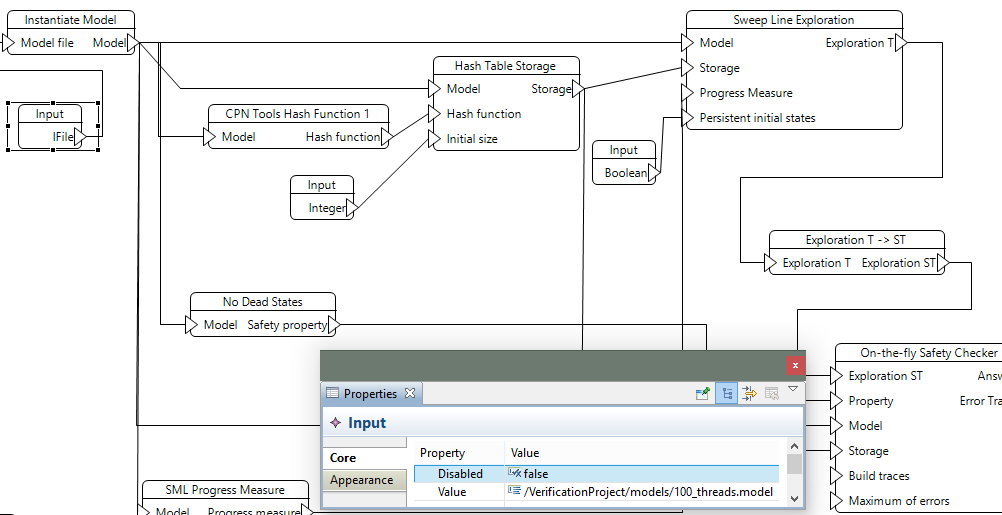
\includegraphics[width=\textwidth]{./img/sl}
	\caption{Sweep-Line Method}
	\label{fig:sl}
\end{figure}

Using the CPN Tools' built-in state space analysis tool, a bounded state space was generated reaching up-to 20 hyperperiods of component thread activity. This bounded generation took 36 minutes on a typical laptop. Our goal with such an example is to evaluate the effectiveness and utility of state space reduction techniques with respect to speed and memory usage. Figure \ref{fig:sl} shows a simple block diagram of the sweep-line method as configured in ASAP. Performing on-the-fly verification checks for lack of dead states in the analysis model, results indicate lack of system-wide deadlocks due to blocking behaviors triggered by RMI-style synchronous peer-to-peer interaction patterns. Figure \ref{fig:ds} shows analysis results obtained from a \emph{Verification Job} executed in the tool. Notice the on-the-fly verification taking less than 10 minutes to perform deadlock checks on this sample deployment. Using the \emph{Palette} in ASAP, several standard ML (SML) user queries can be created to check for domain-specific properties. 

\begin{figure}[h]
	\centering
	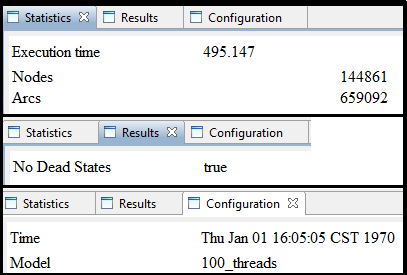
\includegraphics[width=0.6\textwidth]{./img/asap}
	\caption{Dead States Checking in a Component-based application}
	\label{fig:ds}
\end{figure}

It must be noted here that this improved result is due to not only because of the efficient state space search but also because of symmetry-based structural reduction discussed in the previous section. If not for this reduction, the state space search requirements would exponentially grow for each new hardware node added to the deployment. 